%
% ---------------------------------------------------
%
% Trabajo de Final de Grado:
% Author: Gonzalo Jesús García Martín <dracoyue@gmail.com>
% Capítulo: Introducción
% Fichero: Cap4_Herramientas.tex
%
% ----------------------------------------------------
%

\cleardoublepage
\chapter{Herramientas}
\label{chap:tools}

	El software usado ha sido el siguiente:
	\begin{itemize}
		\item {\bf AndroidStudio}\cite{1:androidstudio:online}: Entorno de desarrollo integrado oficial para el desarrollo de aplicaciones para {\it Android}, basado en {\it IntelliJ IDEA}.
		\item {\bf Android}\cite{2:android:online}: Sistema operativo basado en el {\it núcleo de Linux} para dispositivos móviles, televisores, automóviles y relojes inteligentes.
		\item {\bf Firebase}\cite{6:firebase:online}: Proveedor de contenidos que proporciona servicios en la nube de forma fácil y segura, con una integración bastante sencilla con las nuevas tecnologías. Ofrece servicios de recuperación y guardado de datos, registro y acceso de usuarios, reglas de seguridad, simulador y análisis de datos entre otros. Los datos almacenados en este servicio no son datos \href{http://es.wikipedia.org/wiki/SQL}{\textit{SQL}}, si no que son datos \href{http://es.wikipedia.org/wiki/JSON}{\textit{JSON}}\cite{7:json:online}. Sistemas con los que {\it Firebase} está integrado:
		\begin{itemize}
			\item {\bf Android}\cite{2:android:online}: Sistema Operativo para dispositivos móviles propiedad de Google.
			\item {\bf IOS}: Sistema operativo para dispositivos móviles propiedad de Apple Inc.
			\item {\bf Servicios Web}.
			\item {\bf Servicios REST}.
		\end{itemize}
	\end{itemize}
	
	\section{Selección}
	%Por qué seleccionamos las herramientas seleccionadas
	Se ha seleccionado {\it AndroidStudio} por ser un entorno de programación nuevo, de uso intuitivo y ligero en comparación con otros entornos de desarrollo ya existentes que son mas pesados, ya que soportan más lenguajes de programación. {\it Firebase} ha sido elegido por la misma razón, siendo uno de los servicios en la nube más sencillos de utilizar.
	
	\section{Otros entornos de desarrollo integrado: Eclipse}
	Software compuesto por varias herramientas de programación. Éstas son de código abierto multiplataforma para el desarrollo de proyectos. Al ser un conjunto de herramientas, se le considera un entorno de programación integrado, es decir, {\it IDE}.
	
	\subsection{Instalación}
	\begin{itemize}
		\item {\bf JDK}: Descargar e instalar {\it Java Development Kit}\cite{17:jdk:online}.
		\item {\bf JDT}: Descargar e instalar {\it Java Development Tools}\cite{21:jdt:online}.
		\item {\bf Eclipse}: Descargar {\it Eclipse IDE for Java Developers}\cite{15:eclipse:online}.
		\item {\bf Uso}: Descomprimir en la carpeta donde se va a almacenar, y ejecutar {\ttfamily eclipse.exe}.
		\begin{itemize}
			\item {\bf workspace}: Seleccionar donde va a estar el espacio de trabajo en el cuadro de diálogo que aparece al ejecutar Eclipse por primera vez.
			\item {\bf ADT Plug-in}\cite{20:andoirdSDK:online}: Seleccionar {\ttfamily help \textgreater Install new software} y en la ventana que se abre {\ttfamily work with \textgreater add} e introducir la dirección de internet donde se va a buscar los paquetes a instalar.
			\item {\bf Paquetes}: Seleccionar los paquetes de {\it Developers Tools}.
		\end{itemize}
		\item {\bf SDK}: Añadir paquetes {\it SDK} con el gestor de paquetes ({\it SDK Manager}) seleccionándolo en la barra de herramientas (Figura \ref{fig:SdkManager}).
		\begin{figure}[h !]
			\centering
			
\includegraphics{SdkManager}
			\caption{Icono SDK Manager}
			\label{fig:SdkManager}
		\end{figure}
	\end{itemize}
	
	\section{Otros Servicios en la Nube: Parse\cite{16:parse:online}}
	Proveedor de servicios en la nube que ofrece eventos, autenticación de usuarios, almacenamientos de datos, análisis y {\it notificaciones push} entre otros.
	{\it Parse} está integrado con las siguientes tecnologías:
	\begin{itemize}
		\item {\it IOS}.
		\item {\it Android}\cite{2:android:online}.
		\item {\it Javascript}.
		\item {\it OSX}.
		\item {\it Unity}: Software para la creación de videojuegos.
		\item {\it PHP}: Lenguaje de programación.
		\item {\it .Net + Xamarin}.
		\item {\it Arduino}: Hardware libre que consiste en una placa con un microcontrolador y un entorno de programación.
		\item {\it Embedded C}: Lenguaje de programción que extiende sus funcionalidades de C.
		\item {\it Servicios REST}.
	\end{itemize}
	
	\subsubsection{Instalación}
	\begin{itemize}
		\item {\bf Descarga}: Descargar librería de {\it Parse}.
		\item {\bf Librería}: Añadir la librería de {\it Parse} en el archivo {\ttfamily build.gradle} que esta dentro de la carpeta {\ttfamily app} en el directorio raíz del proyecto. Véase listado \ref{code:gradleParse}

		\lstinputlisting[float = h!,language=Java,caption={Importación de la librería de {\it Parse}},label={code:gradleParse}]{Code/buildParse.gradle}
		\newpage
		
		\item {\bf Uso}: En los archivos de clase {\ttfamily  .java}\cite{14:java:online} seguir los siguientes pasos:
		\begin{itemize}
			\item {\bf Librerías}: Importar las librerías necesarias:
			\begin{itemize}
				\item {\bf Cliente Firebase}: Importar la librería del cliente.
				\item {\bf Consultas}: Importar la librería de consultas ({\ttfamily ParseQuery}).
				\item {\bf Listeners}: Importar la librería de oyentes ({\ttfamily FindCallback}).
				\item {\bf Excepciones}: Importar la librería de excepciones ({\ttfamily ParseException}).
				\item {\bf Objetos}: Importar la librería de objetos ({\ttfamily ParseObject}).
				\item {\bf Usuarios}: Importar la librería de atenticación de usuarios ({\ttfamily ParseUser}).
			\end{itemize}
			\item {\bf Claves}: Crear dos contantes de tipo cadena ({\it String}) en las introduciremos manualmente la identificación de la aplicación ({\it AppID}) y la clave del cliente ({\it CLIENT\_KEY}).
			\item {\bf Contexto}: Añadir el contexto en que se va a usar en la función {\ttfamily onCreate()} con la identificación y la clave.
			\item {\bf Consultas}: Preparar la consulta que se va a hacer.
			\item {\bf Oyentes}:Añadir un oyente ({\it Listener}) a la consulta.
		\end{itemize}
		
		En el listado \ref{code:parse} obtenemos un ejemplo de uso de la librería.
		
		\newpage
		\noindent
		\lstinputlisting[language=Java,caption={Ejemplo de uso de {\it Parse}},label={code:parse}]{Code/ParseExample.java}
	\end{itemize}
		
	\section{Instalación de las herramientas usadas}
	En esta sección se procederá a explicar la instalación de {\it AndroidStudio} y {\it Firebase}.
	
	\subsection{AndroidStudio}
	\begin{itemize}
		\item {\bf JDK}: Descargar e instalar {\it Java Development Kit}\cite{17:jdk:online}.
		\item {\bf Descarga}: Descargar {\it AndrodiStudio}.
		\item {\bf Instalación}: Ejecutar el archivo de instalación descargado y seguir los pasos indicados por el instalador.
		\item {\bf SDK}: Añadir paquetes {\it SDK} con el gestor de paquetes ({\it SDK Manager}) seleccionándolo en la barra de herramientas (Figura \ref{fig:SdkManager}).

		\begin{figure}[h !]
			\centering
			
\includegraphics{SdkManager}
			\caption{Icono SDK Manager}
			\label{fig:SdkManager}
		\end{figure}
		\item {\bf Paquetes}: Seleccionar las versiones de {\it Android} \cite{2:android:online} a instalar, se pueden elegir o quitar paquetes concretos de cada versión. Darle a {\it Install}. Es importante que ademas de instalar las versiones a utilizar, se instalen los siguientes paquetes:
		\begin{itemize}
			\item {\it Android SDK Tools}.
			\item {\it Android SDK Platform-tools}.
			\item {\it Android SDK Build-tools} (La versión más actual).
			\item Extras \textgreater {\it Android Support Repository}.
			\item Extras \textgreater {\it Android Support Library}.
			\item Extras \textgreater {\it Google USB Driver}.
		\end{itemize}
	\end{itemize}
	
	En la figura \ref{fig:SdkManager} se pueden observar los paquetes que se pueden instalar.
	
	\begin{figure}[h !]
		\centering
		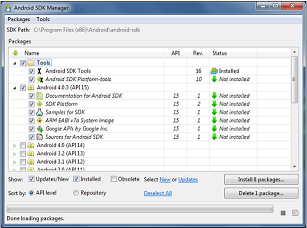
\includegraphics{Packages}
		\caption{Paquetes en SDK Manager}
		\label{fig:SdkManagerPackages}
	\end{figure}
	
	\subsubsection{Primeros Pasos}
	
		Antes de comenzar con el desarrollo de la aplicación, se han implementado varias aplicaciones a modo de ejemplo para afianzar los conocimientos sobre {\it Android}.
		
		\begin{enumerate}
			\item {\it Build your first app}\cite{29:firstapp:online}
			\item {\it Adding the action bar}
			\item {\it Supporting Different Devices}
			\item {\it Managing the Activity Lifecycle}
			\item {\it Building a Dynamic UI with Fragments}
			\item {\it Saving Data}
			\item {\it Interacting with Other Apps}
			\item {\it Sharing Simple Data}
			\item {\it Sharing Files}
			\item {\it Sharing Files with NFC}
			\item {\it Managing Audio Playback}
			\item {\it Capturing Photos}
			\item {\it Printing Content}
			\item {\it Displaying Bitmaps Efficiently}
			\item {\it Displaying Graphics with OpenGL ES}
			\item {\it Animating Views Using Scenes and Transitions}
			\item {\it Adding Animations}
			\item {\it Connecting Devices Wirelessly}
			\item {\it Performing Network Operations}
			\item {\it Syncing to the Cloud}
			\item {\it Transferring Data Using Sync Adapters}
			\item {\it Best Practices for Security \& Privacy}
			\item {\it Best Practices for Testing}
			\item {\it Parse}
			\item {\it Firebase Storage}
			\item {\it Expandable ListView}
			\item {\it TabHost Swipe}\cite{55:tabhostswipe:online}
			\item {\it ActionBar Tab Swipe}
		\end{enumerate}
	
	
	\newpage
	\subsection{Firebase}
	\begin{itemize}
		\item {\bf Librería}: Añadir la librería de {\it Firebase} en el archivo {\ttfamily build.gradle} que esta dentro de la carpeta {\ttfamily app} en el directorio raíz del proyecto. En el listado \ref{code:gradle} se puede observar como se importa la librería de {\it Firebase}.
		
		\lstinputlisting[float = h!,language=Java,caption={Importación de la librería de {\it Firebase}},label={code:gradle}]{Code/build.gradle}
		
		\item {\bf Uso}: En los archivos de clase {\ttfamily .java}\cite{14:java:online} seguir los siguientes pasos:
		\begin{itemize}
			\item {\bf Librerías}: Se han de importar la librerías necesarias:
			\begin{itemize}
				\item {\bf Cliente Firebase}: Importar la librería del cliente.
				\item {\bf Errores Firebase}: Importar la librería de errores en consultas.
				\item {\bf Datos Firebase}: Importar la librería que permite la devolución de datos desde {\it Firebase}.
				\item {\bf Consultas Firebase}: Importar la librería para consultas.
				\item {\bf Librería Oyentes}: Importar la librería de los oyentes ({\it Listeners}).
			\end{itemize}
			\item {\bf Contexto}: Añadir el contexto en que se va a usar en la función {\ttfamily onCreate()}.
			\item {\bf Referencias}: Añadir una referencia a la base de datos o tabla de la misma a la que se van a hacer las consultas.
			\item {\bf Consultas}: Preparar la consulta que se va a hacer.
			\item {\bf Oyentes}: Añadir un oyente ({\it Listener}) a la consulta.
		\end{itemize}
	\end{itemize}

	En el listado \ref{code:firebase} se puede observar un ejemplo del uso de la librería {\it Firebase}.
	
	\lstinputlisting[float = h!,language=Java,caption={Ejemplo de uso de {\it Firebase}},label={code:firebase}]{Code/FirebaseExample.java}